% File naaclhlt2010.tex
% Contact: nasmith@cs.cmu.edu
\documentclass[11pt]{article}
\usepackage{acl-hlt2011}
\usepackage{times}
\usepackage{latexsym}
\usepackage{amsmath}
\usepackage{multirow}
\usepackage{url}
\DeclareMathOperator*{\argmax}{arg\,max}
\setlength\titlebox{6.5cm}    % Expanding the titlebox

\usepackage{arabtex}
\usepackage{amssymb}
\usepackage{caption}
\usepackage{epsfig}
\usepackage{subfigure}
\usepackage{color}
\usepackage{rotate}
\usepackage{rotating}
\usepackage{amsthm}
\usepackage{booktabs}

\usepackage{relsize}
\usepackage{fancyvrb}
\usepackage[colorlinks=false]{hyperref}

\usepackage{utf8}
\setarab
\fullvocalize
\transtrue
\arabtrue


%\newcommand{\CharCodeIn}[1]{`\CodeIn{#1}'}
\newcommand{\CodeIn}[1]{{\small\texttt{#1}}}
\newcommand{\frl}[1]{\fbox{\RL{#1}}} 
\newcommand{\noArRL}[1]{\arabfalse\RL{#1}\arabtrue} 
\newcommand{\noTrRL}[1]{\transfalse\RL{#1}\transtrue} 

%\title{Instructions for NAACL HLT 2010 Proceedings\Thanks{This...}}
\title{Hadith Narrator Chain Extraction using Arabic Morphological Analysis}

%\author{ Jad Makhlouta \\\And
%Hamza Harkous \\
%  American University of Beirut \\
%  {\tt \{jem04, hhh20, fz11\}@aub.edu.lb } \\\And 
%  Fadi Zaraket 
%}

\date{}

\begin{document}
\maketitle
\begin{abstract}
A hadith in Islamic literature is a narration from the 
prophet Mohammad related by multiple narrators.
Establishing the authenticity of a hadith is an important task
in Islamic studies. 
Based on them Islamic scholars issue rules that affect the life
of people around the world. 
The literature lacks an automated exhaustive mechanism of 
authentication checks. 
This is currently manual work prone to error and almost
impossible to complete in the life time of a scholar due to the
large literature available. 
In this paper, we present a tool that uses 
an Arabic application-specific morphological analyzer 
to successfully automate the
analysis of three books of hadith selected 
arbitrarily and abstract 
each book into a graph of narrators related to each other. 
\end{quote}
\end{abstract}

\section{Introduction}

\transfalse
\begin{figure}[tb]
\center{
\resizebox{.9\columnwidth}{!}
{ \input{figs/exhadith.pdftex_t}}
\caption{Hadith abstraction example.}
\label{f:exhadith}
}
\end{figure}
% the FSMs for the three words
\transtrue

A \RL{.hady_t}~\footnote{In this document, 
we use the default ArabTeX transliteration style ZDMG.}
is a narration related to the prophet Mohammad
through a \RL{sanad} or a sequence of narrators. 
The collections of traditions are the second source of
jurisprudence after the \RL{qor'An} for all Islamic schools of thought. 
Figure~\ref{f:exhadith} shows an example \noArRL{.hady_t} in 
Arabic with its transliteration and translation. 
We show proper names in boxes connected
to form complex names of narrators. 
For example, 
\noTrRL{qtybT} is the first name 
of narrator $n_1$, and 
\noTrRL{s`yd} is the name of his father as 
the word \noTrRL{bn} (son of) indicates. 
The sequence of names from $n_1$ to $n_5$ 
constitutes the \noArRL{sanad} 
of the \noArRL{.hady_t}. 
The second part of the \noArRL{.hady_t} is the 
\RL{matn} (content) and constitutes the actual content 
and tradition.

Due to religious and political reasons, 
writing the traditions was forbidden 
until the days of the eighth Umayad Calif,
\novocalize
\RL{`mr bn `bd al`zyz}(717-720 AC), seventy or so years after 
the death of the prophet~\cite{AlAskari}. 
Consequently, many inconsistencies were
introduced to the literature which necessitated 
a thorough authentication study of a tradition before its use in 
jurisprudence.
\vocalize
%An Islamic hadith scholar studies the authenticity of 
%the \noArRL{sanad} of a 
%set of related traditions before using these traditions 
%jurisprudence. 
While different Islamic schools of thought differ on 
how to interpret the content, they almost all agree
that if a \noArRL{sanad} lacks authenticity, 
then scholars can not use the tradition for jurisprudence.

The authenticity of a \noArRL{.hady_t} depends on 
the credibility of the narrators as reported in 
separate biography books. 
The study of \noArRL{.hady_t} authentication is 
currently manual and error prone due to the huge number
of existing traditions and tradition books. 
Hadithopedia~\cite{Hadithopaedia:08}
reports that the tradition and biography
books for one of the Islamic sects amounts to more than 
300 thousand lines of text. 
Al-Azami\shortcite{Al-Azami-91} cites more than eleven books
of digitized tradition books each of several volumes, and a dozen
other biography and secondary authentication books such
as a geographical dictionary of places in hadith. 

In this paper, we present the hadith {narrator chain 
extractor using morphological analysis} (NaCEMA), 
a novel technique that automates
extracting the \noArRL{sanad} from the books of traditions 
into a diagram of chains of narrators. NaCEMA segments
a book into narrations, each narration into its \noArRL{matn} 
and its \noArRL{sanad}, 
and each sanad into its separate narrators. 
This work will lead to 
automate an exhaustive automated \noArRL{.hady_t} authentication 
effort in the future as we plan to 
automatically analyze the biography books.


%Automated analysis of Arabic data sets, including texts, 
%publications, records and digital media is essential
%with the huge digital Arabic content available nowadays. 
\subsection{ Arabic morphological analysis}
Arabic morphological analysis is key to our analysis. 
Current morphological analyzers~\cite{Sughaiyer:04}
use concatenative analysis when
considering the internal structure 
of an Arabic word and
composing it into several {\em morphemes}. 
A morpheme can be a {\em stem}, or an {\em affix}.
An affix can be a {\em prefix, suffix, } or an {\em infix}.
%The analysis of one word may lead to several possible
%morphological solutions.
\vocalize
The word \RL{'a.hmadH}
may have two valid morphological analyses. 
The letter \RL{'a} may be a prefix and the word means 
``I praise him'', or 
%The letter \RL{'a} may also be 
part of the stem \RL{'a.hmad} (a proper noun)
and the word means ``his Ahmad''.

\novocalize
%The accuracy of the solutions suffer due to inherent difficulties
%of morphological analysis of the Arabic language. 
%For example, it is common practice to write Arabic text
%without short vowels. 
%This greatly increases the ambiguity of Arabic text. 
%Arabic letters can have up to 
%four different forms
%corresponding to their position in a word, i.e, beginning,
%middle, end of word and separate forms. 
%This allows the phrase \transfalse
%\RL{il_A\nospace almdrsT} \transtrue
%to be visually recognizable
%as two separate words \RL{il_A} (to) and \RL{almdrsT} (the school) 
%without the need of a space in between. 
%The reason is the first word \RL{il_A} ends with
%\RL{_A} a non-connecting letter. 
%These words,
%referred to as ``run-on'' words~\cite{Buckwalter:04},
%occur often, and greatly increase the
%difficulty of tokenization.

Current morphological analyzers such as 
Buckwalter~\shortcite{Buckwalter:02},
Beesley~\shortcite{Beesley:01},
SAMA~\cite{Kulick:10},
and ElixirFM~\cite{Otakar:07} 
take as input white space delimited tokens~\cite{Kulick:10},
consider them as words,
and enumerate all possible solutions. 
This approach has several problems. 
First, a white space delimited token may have 
more than one word, referred to as ``run-on'' 
words~\cite{Buckwalter:04}.
Second, the exhaustive enumeration may not be efficient and may
not be necessary or appropriate
in some applications as noted in~\cite{Maamouri:10}. 
%Other morphological analyzers such as 
%Amira~\cite{Diab:07,Benajiba:07},
%MAGEAD~\cite{Habash:05}, and MADA+TOKAN~\cite{Habash:09} 
%use machine learning and support vector machines (SVM) 
%to disambiguate the morphological analysis at the expense 
%of efficiency. 
%Xerox rules can be compiled into specialized finite state
%machine (FSM) based analyzers as described in~\cite{Beesley:03}.
%However, the efficiency of the resulting analyzer depends on the
%way the Xerox rules are written. 
%This requires deep knowledge and insight from the user
%in compilation techniques, context free grammars, 
%and morphological analysis.
%context free grammar rules that can be automatically compiled
%into efficient non-deterministic finite state Automata (NDFSA). 

%\subsection{Sarf}
%\label{sec:intro:sarf}

{\bf Sarf.~~~}
In this paper, 
we use Sarf~\footnote{Sarf (name modified for blind review) }
an {\em application-specific efficient
morphological analyzer} that uses 
non-deterministic finite state Automata 
driven by an application-specific controller customized 
by the user. 
%Each machine in Sarf takes one letter at a time as input
%and represents a valid morphological analysis.
The application-specific controller prunes false positives
early in the run by making a decision at every input letter
to control the machines.
Sarf builds on and extends the lexicon of Buckwalter~\shortcite{Buckwalter:02} 
with proper and location names extracted from different online 
sources~\footnote{\href{http://alasmaa.net/}{http://alasmaa.net/ }, 
\href{http://ar.wikipedia.org/}{http://ar.wikipedia.org/}}
%as well as biblical sources~\footnote{Genesis 4:17-23; 5:1-32; 9:28-10:32; 11:10-32; 25:1-4, 12-18; 36:1-37:2; Exodus 6:14-25; Ruth 4:18-22; 1 Samuel 14:49-51; 1 Chronicles 1:1-9:44; 14:3-7; 24:1; 25:1-27:22; Nehemiah 12:8-26; Matthew 1:1-16; Luke 3:23-38}.
as well as biblical sources.
%~\footnote{Genesis 4:17-23; 5:1-32; 9:28-10:32; 11:10-32; 25:1-4, 12-18; 36:1-37:2; Exodus 6:14-25; Ruth 4:18-22; 1 Samuel 14:49-51; 1 Chronicles 1:1-9:44; 14:3-7; 24:1; 25:1-27:22; Nehemiah 12:8-26; Matthew 1:1-16; Luke 3:23-38}.

%Each alive machine in Sarf takes as input one letter at a time 
%from a text stream. 
Sarf does not assume that the word at hand is a token and
performs tokenization on the fly based on morphological correctness
and thus can handle 
the ``run-on'' words problem. 
Sarf also uses diacritics if they exist to disambiguate 
morphological solutions. 

%The hadith 
%application specific controller that controls Sarf considers 
%proper names and ignores text where
%proper names occur rarely.
%It also considers words that relate names to each other 
%such as \RL{bin} or ``the son of''
%and words that mean narrate such as \RL{qaal} or ``said''. 

%With Sarf, we successfully automated the analysis of 
%three books of Islamic narrations~\cite{IbnHanbal,AlTousi,AlKulayni}
%and extracted from each one of them a vector of complex structures 
%that are three level deep in hierarchy.
%We also merged these vectors into a graph of narrators where 
%we represented identical narrators from separate traditions 
%in one single node. 

%The rest of this paper is structured as follows. 
%In Section~\ref{sec:sarf}
%we discuss Sarf and illustrate it with a running example.
%We also explain how non-deterministic finite state Automata
%work. 
%In Section~\ref{sec:islamic} we present the hadith application. 
%We present our results in Section~\ref{sec:results}.
%In Section~\ref{sec:related}
%we compare NaCEMA to related work. 
%We conclude with future work in Section~\ref{sec:future}.

%\section{Background}
% TODO: nondeterministic finite-state automata



%The survey in~\cite{Sughaiyer:04} compares
%several morphological analyzers. 
%Analyzers such as~\cite{Khoja:01,Darwish:02} 
%target specific applications in the 
%analyzer itself or use a specific set of POS tags
%as their reference.
%Sarf differs in that it is a general morphological 
%analyzer that reports all possible solutions. 
%It is case-based in the sense that a controller 
%prunes these solutions. 
%
%Sarf builds upon the lexicon of Buckwalter\shortcite{Buckwalter:02}.
%It differs from Buckwalter in that it defines a shorter list of affixes
%and a longer list of affix compatibility rules to allow 
%affixes to be defined recursively
%so that we can have prefix-prefix an suffix-suffix 
%concatenations.
%This allows Sarf to better maintain and propagate 
%the POS tags associated with affixes. 
%%This information is highly 
%%redundant with Buckwalter.% and that may lead to consistency issues. 
%Sarf keeps all the possible analyses alive where each analysis
%corresponds to a set of decisions and positions in the text. 
%Buckwalter produces a set of solutions for each token 
%and the several analysis threads of the text need to be 
%generated as a product of the token solutions. 
%
%Similar to Sarf, Beesley~\shortcite{Beesley:01} uses
%finite state Automata (FSA). 
%It reports that the number of Automata generated by a compiler
%for Xerox rules can not be controlled and also reports a difficulty 
%to compose the FSAs into a single framework. 
%Sarf however constructs an NDFSA from
%the controller and the prefix, stem, and suffix deterministic 
%transducers to solve the problem.
%Sarf also differs in that it uses recursive affixes in the 
%affix transducers, and in that the transducers consider
%input from the controller to modify their behavior. 
%%With Sarf it is easy to control the FSA with a case-based
%%controller. 
%Beesley requires recompilation of the Xerox rules.
%
%Similar to The MADA+TOKAN toolkit, Sarf thinks of
%the several valid morphological analyses as a richness that 
%should be exploited at a higher abstract level rather than
%an inaccuracy that should be corrected. 
%Sarf differs in that it provides an interface for the 
%case study to interfere in judging the analyses much earlier and
%at a finer granularity level. 
%In Sarf, there is no need for a separate tokenizer such as
%TOKAN since each solution keeps a stack of positions
%that partition text into morphemes.
%%The case-based controller can build the trace 
%%when needed. 
%
%%MAGEAD 
%%Maamouri, Mohamed and \bgroup et al.\egroup },
%
%Our approach is close to the refinement of SAMA~\cite{Maamouri:10}.
%SAMA was refined to interact with
%the ATB~\cite{Maamouri:04} project after the addition of a large 
%new corpus. 
%%We find supporting evidence in this decision to our hypothesis
%%about the utility of a case-based analyzer. 
%The algorithmic changes in SAMA were
%done manually and worked in integration with the ATB format. 
%Sarf is a case-based controller approach that can modify 
%the behavior of the analyzer on the fly and can interact
%with any case study. 
%%In Sarf, the analyzer remains general, and the 
%%case-based controller specializes the analysis.
%
%The AMIRA~\cite{Diab:07} analyzer uses 
%a language independent SVM based analysis. 
%The SVM analysis learns features from the input text 
%and does not make use of any information 
%in the target query.
%
%Like ElixirFM~\cite{Otakar:07}, Sarf builds on the lexicon
%of the Buckwalter analyzer. 
%Sarf also uses deterministic parsing with tries 
%to implement the affix and stem transducers. 
%We think that the inferential-realizational approach 
%of ElixirFM
%that is highly compatible with the Arabic linguistic 
%description~\cite{Badawi:04}
%can benefit from many features unique to the Arabic language.
%Sarf leaves implementing that to the case-based controller
%since in many cases the abstraction needs only a partial 
%linguistic model of the Arabic language. 
%%We can compare the case-based controller in Sarf to a high level
%%component in the ElixirFM domain specific language. 
%

%Sarf encodes the prefix, suffix and stem lexicons into
%three deterministic transducers and 
%uses a non-deterministic construction
%of the three to compute all valid morphological analyses.
%We first present a running example of Sarf.
%The running example explains how Sarf works,
%implements recursive affixes, and
%handles ``run-on'' words.
%Then we discuss how Sarf builds and composes the different FSAs.

\section{Narrator chain extraction }
\label{sec:islamic}

%Several researchers~\cite{Hadithopaedia:08} attempted to automate 
%the analysis of the hadith literature. 
In this paper, we use Sarf to successfully automate the
analysis of three books of hadith selected 
arbitrarily~\cite{IbnHanbal,AlKulayni,AlTousi}\footnote{We obtained
  the digitized books from online sources such as 
  \href{http://www.yasoob.com/}{http://www.yasoob.com/} and 
  \href{http://www.al-eman.com/}{http://www.al-eman.com/}. }
%  Our understanding is that those books are historical documents with 
 % public IP.}.
%\setcode{utf8}
%\begin{arabtext}
%حدثنا \emphasize{هشيم}، أخبرنا \emphasize{إسماعيل بن أبي خالد}،
% عن أبي إسحاق، عن سعيد بن جبير، قال كنا
%    مع ابن عمر رضي الله عنه حيث أفاض من
%    عرفات إلى جمع فصلى بنا المغرب ومضى
%\end{arabtext}
%\setcode{standard}
NaCEMA accepts a book as input
and segments it into a vector of hadiths. 
NaCEMA segments each hadith into its
sanad and matn parts. 
NaCEMA 
detects the chain of narrators in the sanad and 
the relation that links each narrator to his ancestor and 
predecessor in the chain. 
It also detects the full name of each narrator that is
composed of several proper names with connectors
in between. 


\subsection{The hadith controller}
\label{sec:controller}
% FSM for the controller

Intuitively, the controller reports a valid chain 
of narrators when a sequence of names
connected by narrator connectors appears. 
This includes the task of finding multi-word names
such as \RL{`bd alr.hmn} often appearing as ``run-on'' words.
The controller marks the beginning of the hadith with the beginning of 
the current proper name sequence,
and marks the end of the hadith with the beginning of the 
next proper name sequence. 
It detects the chain of narrators as the sequence itself. 

%The controller also targets words that mean ``narrate'' when
%they appear between proper names. 
We illustrate the hadith controller 
in Figure~\ref{f:hadith}. 
The transitions are labeled by outputs generated from 
the Sarf morphological analyzer that correspond to 
part of speech (POS) tags. 
A NAME label denotes a proper name.
An NRC label denotes a narrator connector such as
\RL{`an} ``on behalf of'', \RL{.hada_t} ``narrated'', \RL{qaal} ``said'', 
\RL{'a_hbar} ``told'' or one of their morphological equivalents. 
An IBN label denotes the word \RL{ibn} ``the son of'' and is a name connector.
A NISBA is a possessive adjective that qualifies a person such 
as \RL{alma.sriy} ``the Egyptian''. 

The symbol $\tau_{\mbox{NMC}}$ is a threshold
that corresponds to the number of tolerated name connectors 
that may occur between two names. %3
The symbol LIST$_{\mbox{NMC}}$ corresponds to the list 
of name connectors collected since the controller
started looping in the state NMC\_S. 
The symbol $\lambda_{\mbox{NMC}}$ is a parameter 
that corresponds to a relaxed tolerance measure that
the controller resorts to in case the words separating
two names were longer than $\tau_{\mbox{NMC}}$ but 
contained a name connector word such as IBN or NISBA.

The controller has four states that correspond to 
a position in text relative to the next sanad. 
State TEXT\_S is the initial state and denotes that
the controller is outside the context of a sanad.
The controller moves to state NAME\_S on
NAME.
State NRC\_S means that the controller is in the context
of a narrator name after Sarf reports an NRC.
State NMC\_S
indicates that the controller expects a name to appear within 
a tolerance threshold expressed by 
$\tau_{\mbox{NMC}}$ and $\lambda_{\mbox{NMC}}$.

Similarly, the NRC\_S state tolerates $\tau_{\mbox{NRC}}$ words 
before it gives up on its expectations. 
We reach the NAME\_S state only when a
valid NAME is detected and we leave when no more NAME's are detected.
The NRC\_S state can only be reached if an NRC is detected.
NMC\_S can only be reached from a NAME\_S state.
We used the values of 3, 5 and 5 for $\tau_{\mbox{NMC}}$, 
$\lambda_{\mbox{NMC}}$, and $\tau_{\mbox{NRC}}$ respectively.

\begin{figure}[tb!]
\center{
\resizebox{.9\columnwidth}{!}
{ \input{figs/hadith.pdftex_t}}
\caption{The controller of the hadith application.}
\label{f:hadith}
}
\end{figure}

%The definition of input labels such as NAME and IBN depends on the 
%morphological analyzer. 
%However, our case-based controller approach was able to perform well
%under both Sarf and a refined version of Sarf.

\section{The narrator graph}

\begin{figure}[tb]
\center{
\resizebox{1.1\columnwidth}{!}
%{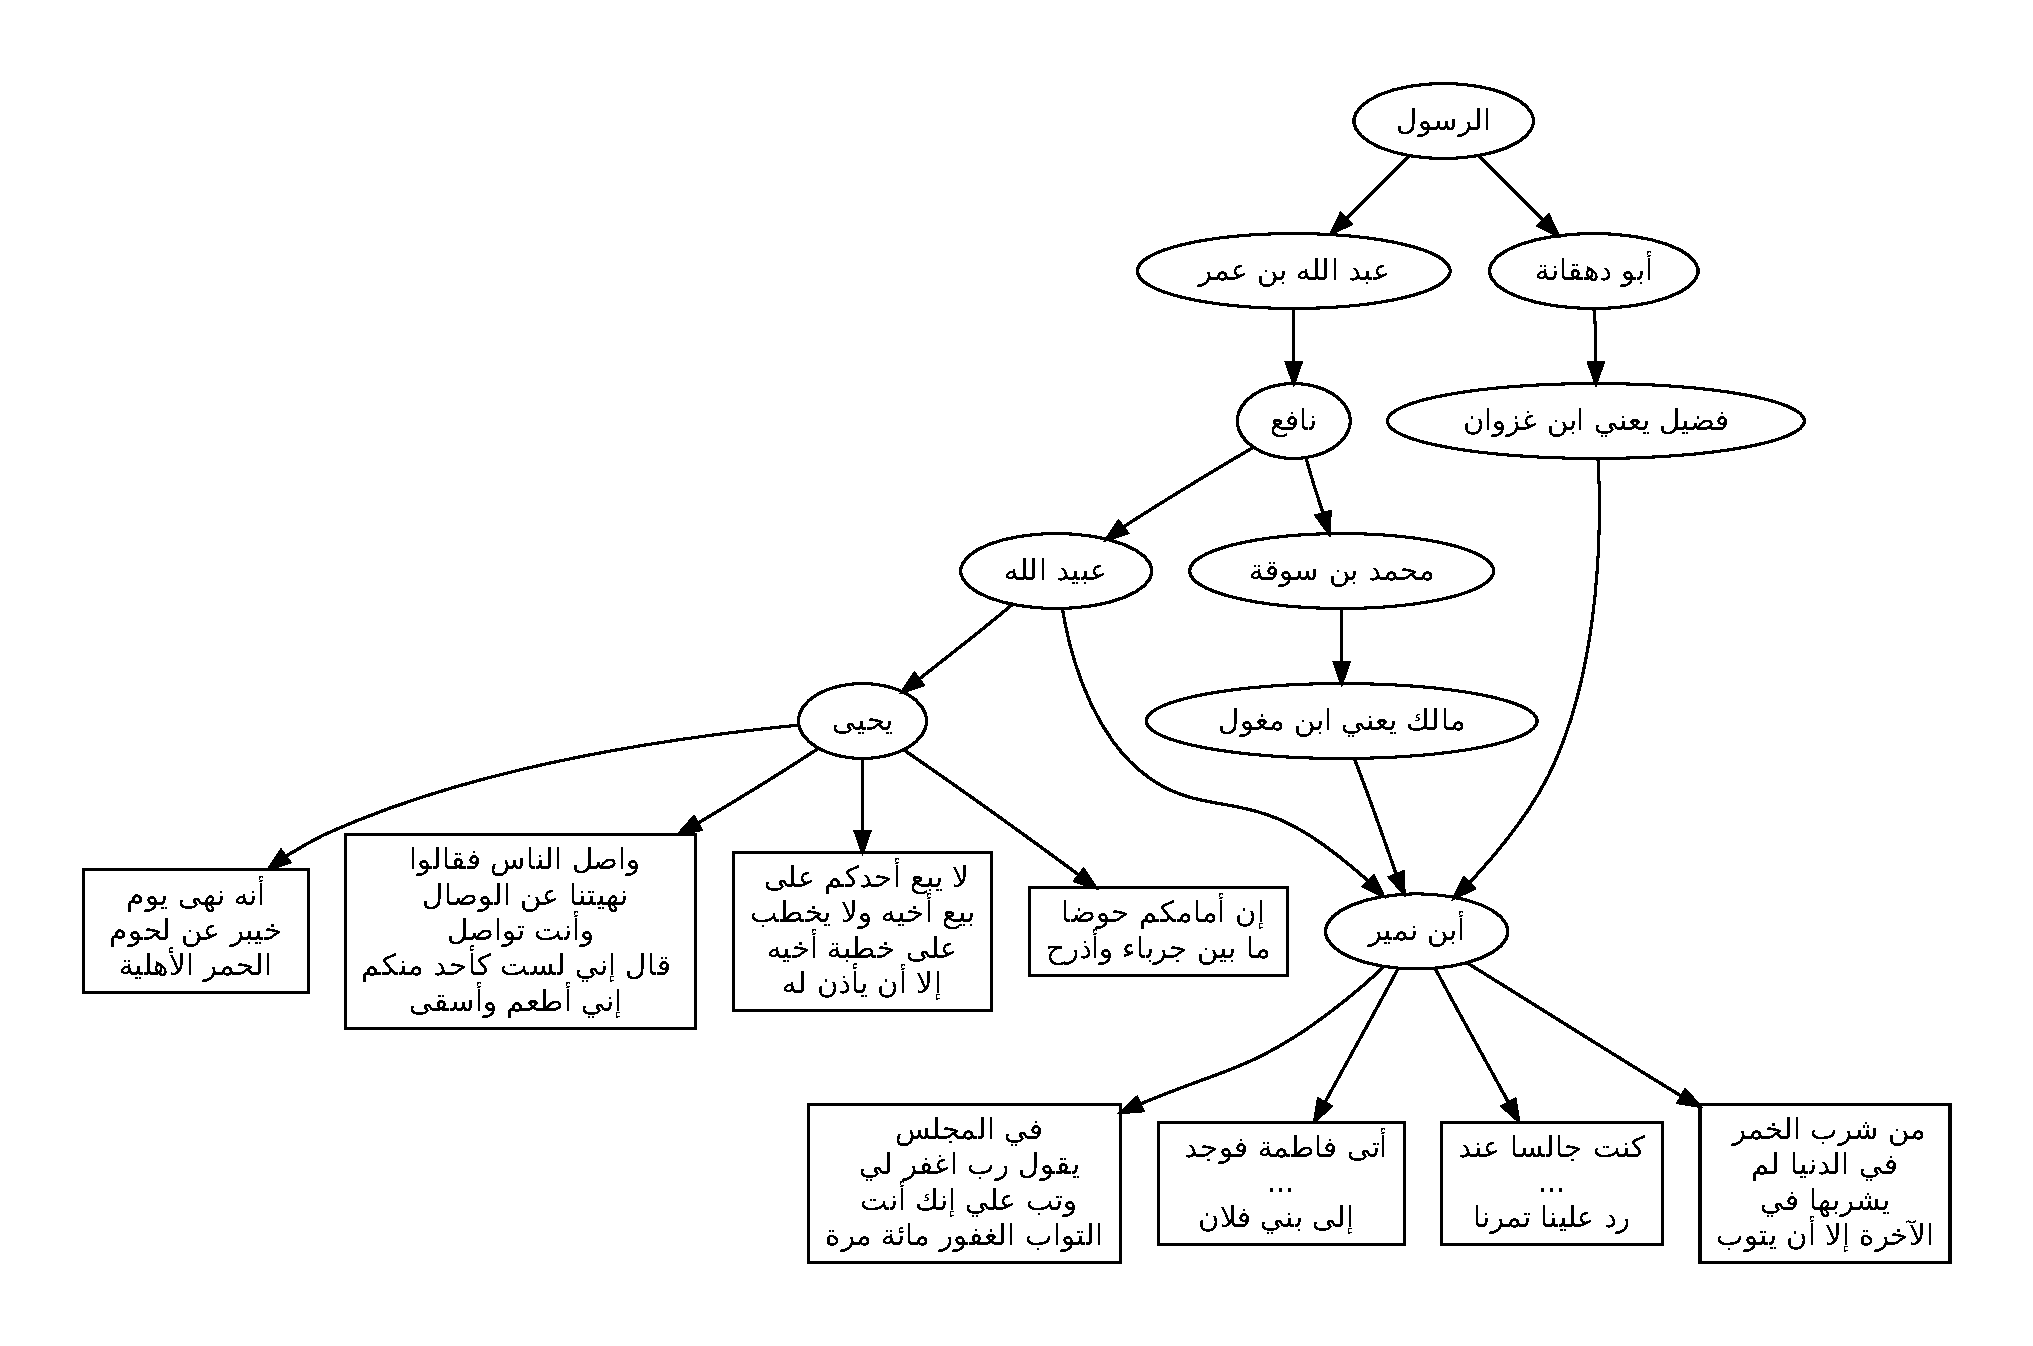
\includegraphics{figs/narrator_chain_output.pdf}}
{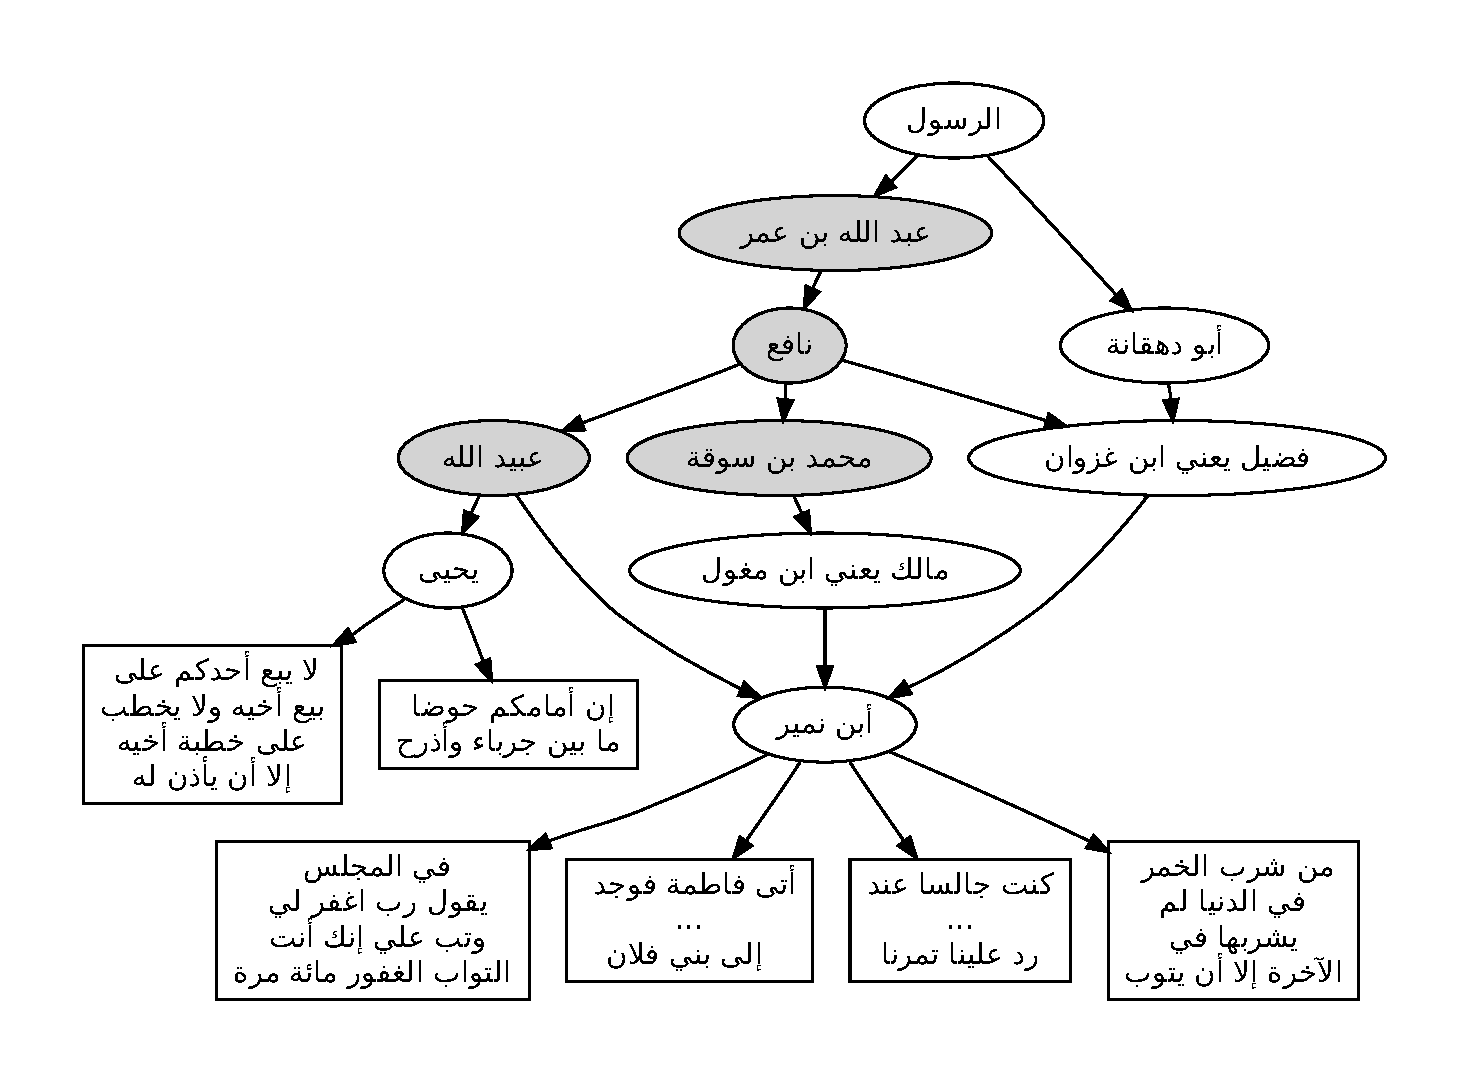
\includegraphics{figs/DAG_narrator.pdf}}
\caption{Narrator directed acyclic graph 
    extracted using NaCEMA }
\label{f:narrators} 
}
\end{figure}

The directed acyclic graph (DAG) 
in Figure~\ref{f:narrators} shows a partial order relation (POR) 
between narrators.
We automatically extracted the POR from three books of hadith 
selected arbitrarily~\cite{IbnHanbal,AlKulayni,AlTousi}.
The nodes in boxes are the \RL{matn} of the hadith, 
and the other nodes are the narrators.
Given a set of chains of narrators similar to 
Figure~\ref{f:exhadith} we formed the DAG using graph algorithms 
that merged equal names in the chains. 
We compared the narrators together using a morphological
distance function. 
We considered each narrator to have several morphological 
components and we rewarded every morphological match with 
a small $\delta$. 
Then we apply a threshold $\tau$ to the sum of rewards
decide the equality of the two narrators. 
We omitted the details of the distance function for brevity.

\section{Results}
\label{sec:results}

\begin{table}[bt]
\centering
\caption{Results of the hadith case study with Sarf.}
%\begin{tabular}{|p{1.5cm}||c|c||c|c||c|c|} \hline
\resizebox{1.1\columnwidth}{!}{
\begin{tabular}{lcp{.2cm}cp{.2cm}c} %\cline{2-10}
 &  AlKafi & & AlIstibsar & &IbnHanbal \\ \cline{1-6}
Word count  &98,943 & & 103,835 & & 20,354 \\ 
 Names       & 12,060  & & 14,613& & 3,013\\
%Names/Narrator & 1.97 & & 1.84& & 1.25 \\
Narrators  & 2,623 & & 5,767& & 1,755 \\ 
%Narrators/Chain  & 4.84 & & 4.76 & &4.05 \\
Chains  & 542 &  & 1,211& & 433 \\ 
Ignored names  & 6,400 &  & 3,348 & & 642 \\ \hline
Segmentation accuracy  & 96\%& & 96\%& & 92\%\\ 
Chain accuracy & 99\%&  & 99\%& & 97\% \\ 
%Narrator accuracy  & & & & &  & & & \\ 
Narrator accuracy  & 91\%& & 90\% & & 90\% \\ \hline
%Name false positives  & 7\%&  & 4\% & & 4\% \\ \hline
Running time (secs.)& 1.32 & & 1.31 & & .096\\ \hline 
\end{tabular}
}
\normalsize
\label{t:hadithresallresults}
\end{table}

We ran our experiments using a dual core 2.66 Ghz 64-bit processor 
with 4GB of memory using a Linux operating system. 
We report our results in Table~\ref{t:hadithresallresults} on the 
three hadith books.
NaCEMA detected narrator chains and segmented the books 
correctly with an accuracy above 90\%
in all cases and across all the traditions in the three books. 

The row for ``word count'' is an indicator of the size of the data.
The %numbers in 
rows ``names'', ``narrators'', and ``chains'' denote the total
number of the corresponding entities per book.
The row ``ignored names'' reports the number of names detected 
outside the chains and thus are irrelevant to
the application. 
%In addition, the rows ``names/narrator'' and ``narrators/chain'' 
%report the average
%number of names per narrator and 
%the average number of narrators per chain respectively. 

The ``segmentation accuracy'' reports on the accuracy of 
segmentation of the book into separate hadiths.
We computed the metric manually by marking the beginning 
and end of a representative sample of hadiths in each 
book and compared that to the NaCEMA results. 
We used the same approach to compute all other accuracy measures.
The ``chain accuracy'' reflects the percentage of correct narrators 
covered by extracted chains.
The ``narrator name accuracy'' row reflects the percentage of 
correct proper names detected within
narrator structures.

%The row ``name false positives'' reports the percentage of words 
%recognized as names while they should not.
%We notice that this metric did not affect the accuracy
%of narrator and chain segmentation since detecting
%a narrator or a chain with the refined analysis without substantially affecting the 
%high abstract measures such as chain and segmentation
%accuracy.

\section{Related work }
\label{sec:related}

The closest to our work is e-Narrator~\cite{Azmi2010}, a 
tool that uses a grammar based approach to solve 
the narrator extraction problem. 
The e-Narrator tool preprocesses the text to remove 
punctuation and diacritics and to normalize white
spaces. 
Then e-Narrator uses a similarity-based approach
to memory based learning~\cite{Azmi2010} in order to perform 
shallow parsing of the preprocessed text. 
The e-Narrator tool uses a parser based on a context
free grammar that enumerates several ways to express
the name of the prophet, several possible words that 
might precede the name of the prophet, several possible
words that might separate two narrators, and several
words that might separate parts of the name of the narrators.
The e-Narrator tool fails when a variation of one of the 
listed words and not an exact form of it
happens in the text. 
In their grammar they consider a name to be any sequence of 
legal Arabic characters. 
The e-Narrator tool generates successfully 86.7 percent of
the narration chains of 90 selected traditions with 
34 simple cases and 56 hard cases. 

NaCEMA does not need a preprocessing step since 
it uses morphological analysis to process the text. 
While e-Narrator bases its analysis on the patterns 
of words that surround the narrator names, 
NaCEMA bases its analysis on the fact that narrator
names are likely to happen in localities with a high
number of proper names. 
NaCEMA uses the narrator connectors as helpers and
uses morphological analysis to compare the stems of
those words and thus NaCEMA avoids the problem of 
``parser noise words'' that e-Narrator faces. 
Even though we do not have access to the selected
90 traditions e-Narrator reports on, we claim
that NaCEMA outperforms e-Narrator as it works on
the full text of the presented hadith books
and reports a higher success rate. 


\section{Conclusion and future work}
\label{sec:future}

We presented NaCEMA, a narrator chain extractor
using morphological analysis. 
NaCEMA extracted narrator chains with above 90\% accuracy
from three different hadith books and generated 
directed acyclic graphs relating the narrators 
in a partial order relation. 

This partial order graph is instrumental to automate
localization of narrators in biography documents and
segmenting biography documents in the future.
Given that a biography discusses a narrator 
and mentions his professors and students,
we plan to segment the biographies with a graph 
coloring algorithm
that traverses the text and colors the POR whenever
a name is found. 

Once the biographies are analyzed, we can annotate
the POR with qualifiers of the narrators that reflect
their authenticity. 
%We can also annotate the POR with the locations and 
%the time the narrators lived in. 
%Then we can compute a time and location overlap
%check to discover inconsistent narrations.
%We can also perform several interesting checks using 
%this POR on its own such as checking for the effect of
%one narrator on the hadith literature. 

We also plan to 
enhance the accuracy of hadith detection and the 
narrator merging algorithms. 

%We plan to make use of the name connector and narrator
%connector stop phrases that our case study extracted to create a 
%learning system that can learn more names. 
%We also plan on developing an Arabic linguistic computational model 
%similar to that of ElixirFM~\cite{Otakar:07} but that can be 
%explored partially based on the case study. 

%\section{Acknoledgements}
%\label{sec:acc}
%We thank the Lebanese National Council for Scientific Research (LNCSR) for funding this research.


%For reasons of uniformity, Adobe's {\bf Times Roman} font should be
%used. In \LaTeX2e{} this is accomplished by putting

%\begin{quote}
%\begin{verbatim}
%\usepackage{times}
%\usepackage{latexsym}
%\end{verbatim}
%\end{quote}
%in the preamble.

%Additionally, it is of utmost importance to specify the {\bf
%  US-Letter format} (8.5in $\times$ 11in) when formatting the paper.
%When working with {\tt dvips}, for instance, one should specify {\tt
%  -t letter}.

%{\bf Citations}: Citations within the text appear
%in parentheses as~\cite{Gusfield:97} or, if the author's name appears in
%the text itself, as Gusfield~\shortcite{Gusfield:97}. 
%Append lowercase letters to the year in cases of ambiguities.  
%Treat double authors as in~\cite{Aho:72}, but write as 
%in~\cite{Chandra:81} when more than two authors are involved. 
%Collapse multiple citations as in~\cite{Gusfield:97,Aho:72}.


%\section*{Acknowledgments}
% this will go into the regular submission

%\bibliographystyle{naaclhlt2010}
\bibliographystyle{acl}
{\small \bibliography{fzAr}}

\end{document}
